RLDM begins! Today we have tutorials split between

\subsection{Tutorial by Melissa Sharpe: Testing Computational Questions via Associative Tasks}

\dbox{Main claim: We can use associative tasks to test computational questions.}

A few disclaimers: 1) I am not a computational neuroscientist, but rather a behavioral neuroscientist! 2) Not the first person in the field to make this claim. \\

Outline:
\begin{enumerate}
    \item Some basic principals of associate learning.
    \item Computational account of dopamine prediction error.
    \item a few associative tests of the computational account.
    \item Towards a new theory.
\end{enumerate}


\subsubsection{Overview: Associative Learning}


\ddef{Associative Learning}{The way we form associations between stimuli/experiences in our environment.}

If we can better understand this process, we can start to shed light on how we perform much more complex reasoning, inference, and modeling. \\

$\ra$ Will mostly be seeking this understanding from the perspective of the rat (as in classical Pavlovian conditioning studies). \\

{\bf Idea:} Deliver different stimuli (auditory tones of different length/pitch), then deliver different foods (that rats like). \\

$\ra$ Over time, rats will learn to associate food with different tones, and their behavior will reflect this. \\

{\bf Key Finding:} Crucially, prediction error is a catalyst for learning. Will not go to the place food is delivered when light (a new stimuli) is presented. \\

Q: So, what is the qualitative nature of what the animals have learned, when a note is presented? Why do the rats go to the food cup? \\

A: If we pre-feed an animal with food and present the tone, they {\it wont} go to the food~\cite{rescorla1982behavioral}. So: not just a value based decision, but a sensory specific representation that binds the stimuli of the tone to the food (not just reward). \\

But! There is still a response that is more purely value based. A rat will happily pull a lever that generates the tone (even if it doesn't lead to food). \\

Two forms of learning:
\begin{enumerate}
    \item Development of association between tone and specific food it predicts.
    \item Tone also accrues general value that is independent of the desire for the food.
\end{enumerate}

$\ra$ Powerful dichotomy! People with drug addictions show a change in the balance between these associations~\cite{everitt2005neural}. \\

Neutral associations: learn about the general structure of the environment even when not attached to motivation (reward learning). \\

$\ra$ A rate may learn tone and light co-occur. Then, if just the tone is played and the food is given, the rat will {\it also} associate food with the light! \\

$\ra$ Great procedure for understanding how rats/animals learn about these kinds of neutral associations. \\

Summary of basic principles:
\begin{itemize}
    \item Pavlovian conditioning has two forms of learning: 1) associative, and 2) accrual of value
    \item Small changes to task design have big consequences for underlying associations
    \item Sensory preconditioning: isolates associations between events.
    \item Second-order conditioning: isolates cue value.
    $\ra$ Lets us probe which brain regions contribute to specific aspects of learning.
\end{itemize}

\subsubsection{Computational Theory for Understanding Learning}

Dopamine prediction error (DPE):
\begin{itemize}
    \item Early experiments by \citet{schultz1997neural} led to the finding of the DPE
    $\ra$ Dopamine neuron errors signal in expectation.
    
    $\ra$ Old experiment: animals' dopamine neurons fire right after receiving tasty juice. Then, if the animal expects the signal but doesn't get it, there's a retraction (error prediction). See results in Figure~\ref{fig:dopamine}.
    
    \item Widespread across different kinds of animals, intimately connected to reward learning in many species.
\end{itemize}

\begin{figure}[h!]
    \centering
    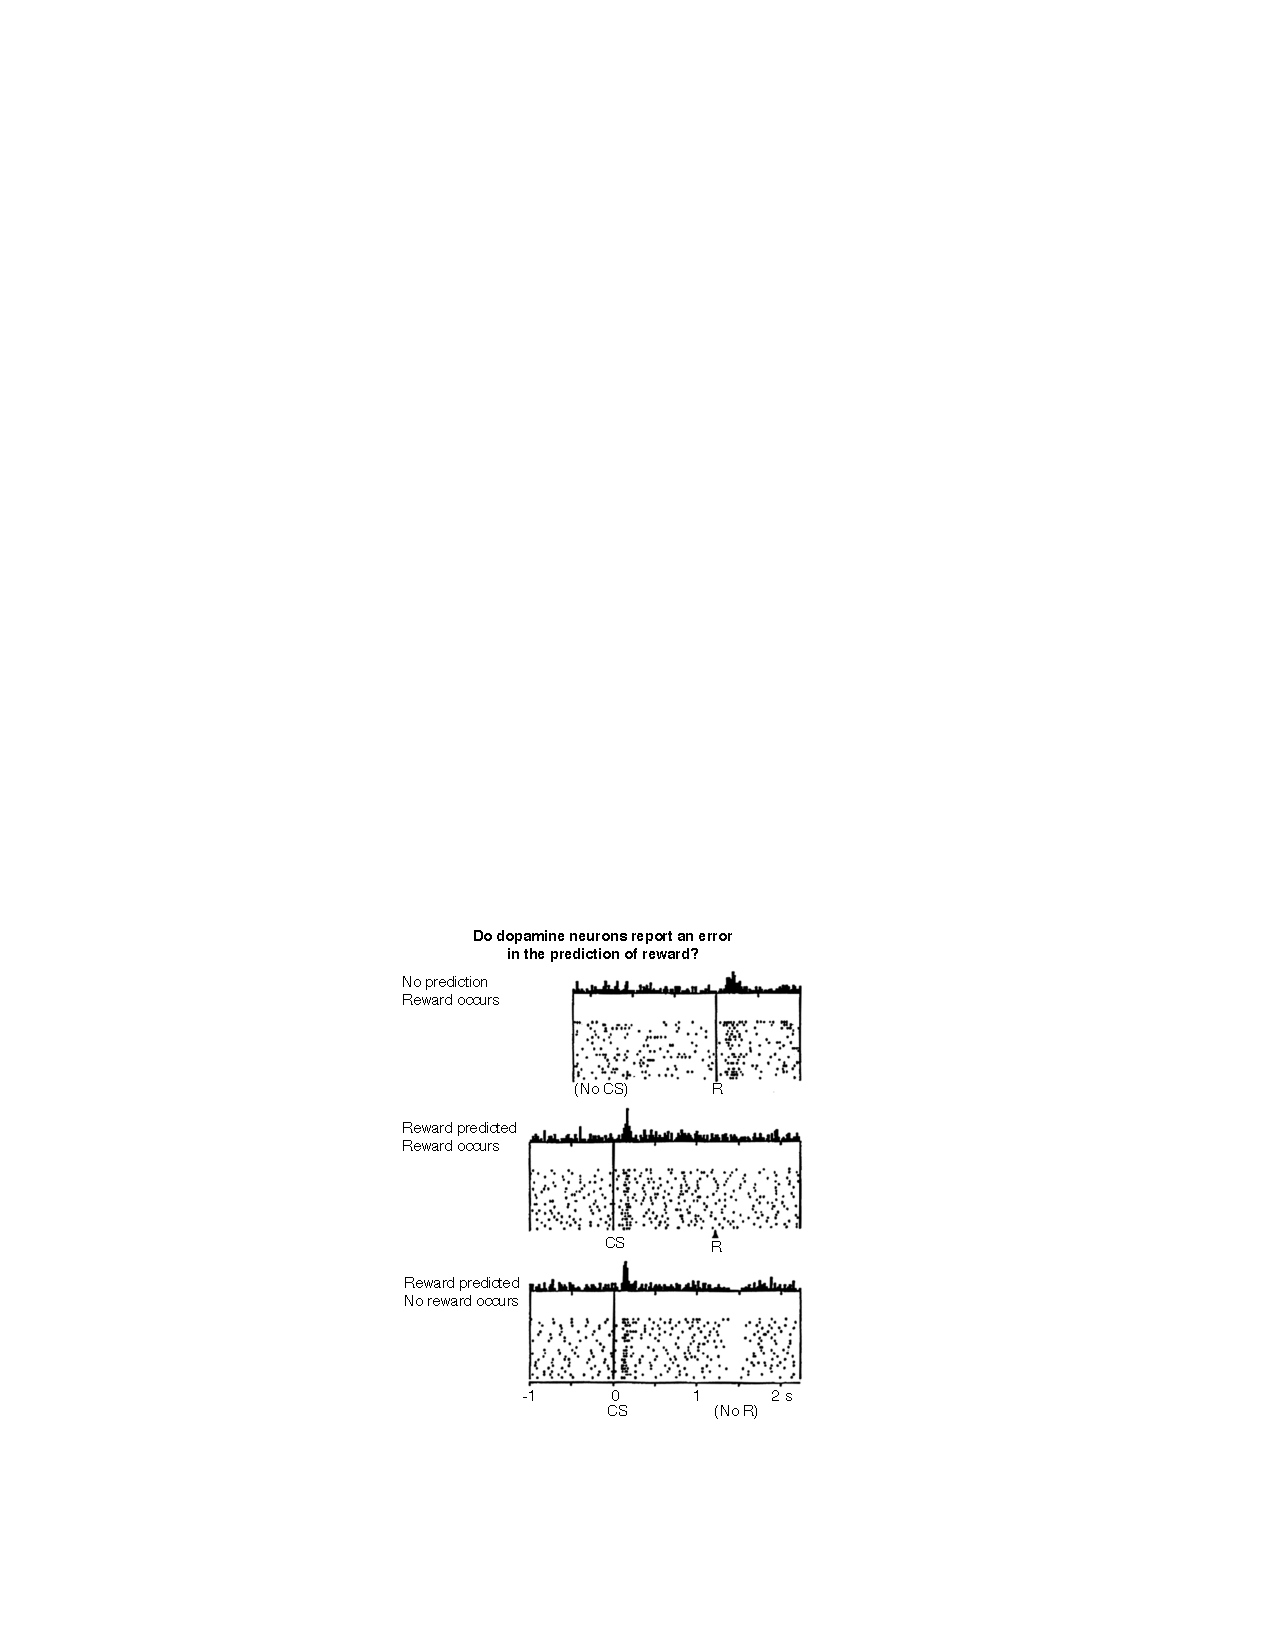
\includegraphics[width=0.4\textwidth]{images/dopamine.pdf}
    \caption{Results from \citet{scheessele18frame} on the dopamine prediction error.}
    \label{fig:dopamine}
\end{figure}


Computational account: Temporal Difference error
\[
\Delta V = \alpha \delta(t),
\]
with $\delta(t)$ the error in value prediction:
\[
\delta(t) = r_t + \gamma V(s_t) - V(s_{t_1}).
\]

Dopamine: believed to play the role of attributing value to stimuli. \\

Summary: 1) dopamine neurons fire when error in expectation, 2) Functions to assign value to the cue antecedent to rward, and 3) Does not function to produce associations to cue reward. \\

But! New theory: optogenetic revolution~\cite{roesch2007dopamine}. \\

\subsubsection{Experiments on Understanding Dopamine}

$\ra$ One idea: stimulating dopamine unblocks (avoids being distracted by surprise) learning~\cite{steinberg2013causal}. \\

Test: contrast time spent by rats looking for food with and without dopamine stimulation during a sensory stimuli (like the light/sound).


Conclusion: dopamine drives learning! But, we don't know yet how. \\

$\ra$ Next experiment explores how. \\

Main Q studied: What is the role of dopamine in learning? \\

Experiment~\cite{keiflin2019ventral}:
\begin{itemize}
    \item (Control Group) Increase reward unpredictably when stimuli is presented contrasted with predictable dopamine stimulation.
    $\ra$ Control: A yields more sucrose than B. But then, A and AX yield same reward, whereas B and BY have a difference (BY gives more sucrose than B)
    
    $\ra$ Dopamine stimulation group: train A and B with same magnitude of reward. So, learning about Y in this 2nd group should be {\it blocked}. Won't learn about Y because it predicts the same as B.
    
    \item So, studying whether dopamine unblocks learning.
    
    \item Then: devalue the outcome by taking the rat outside of the chamber and let them eat as much sucrose as they'd like (and give them a tiny dose of lithium to make them slightly sick).
    
    $\ra$ Finding: so, dopamine is an integral part of this unblocking process in learning, not just value learning.
\end{itemize}

Experiment on model-based learning~\cite{sharpe2017dopamine}
\begin{itemize}
    \item Introduce $A\ra X$ association (where $X$ is rewarding), then $AC\ra X$ association.
    $\ra$ Association with $C$ is blocked if $A\ra X$ is learned first!
    \item Can even add $EF \ra X$ association, which rats should learn since they have never seen $E$ or $F$. At the same time, rats will be given $AD \ra X$ and $AC \ra X$. 
    
    \item Finding: Animals learn $x$ leads to reward (go to find the food), do {\it not} learn about $C$ or $D$, but do learn about $EF$ when no dopamine is stimulated.
    
    $\ra$ When dopamine is stimulated, they do learn about $C$ (dopamine unblocks $C$).
\end{itemize}

{\bf Key takeaway:} dopamine drives learning of associations between cues and events.


Next experiment: stimulate dopamine during a cue that doesn't do anything~\cite{saunders2018dopamine}. Contrast paired/unpaired groups where dopamine is stimulated right after a light is turned off vs. a minute later (effectively uncorrelated to the rat). \\

Q: Will the paired groups pull a lever to get the light to turn on?

$\ra$ Finding: Yes! Suggests dopamine can associate value between stimuli, too. But, further finding (from the same lab) suggests that the opposite can be true too, under the right conditions. \\

{\bf Question to leave with:} Why should we care that in some conditions, dopamine can assign value to a cue, while in others, it doesn't? \\

A: This is really important for our understanding of pscyhopathology! Schizophrenia and drug addiction are both characterized by disruption in midbrain dopamine systems, but they're very different disorders. \\

$\ra$ Schizophrenia could be a disorder characterized by dopamine dysfunction during learning (while addiction is not). \\

Summary:
\begin{itemize}
    \item Revealed that dopamine error contributes in a causal manner to learning
    \item Really small changes in your task can have really big consequences for the associations underlying it!
\end{itemize}

\spacerule

%Q: common views about how consistent the role of dopamine is across the animal kingdom? key ways in which it might differ?

\subsection{Tutorial by Cleotilde Gonzales: Dynamic Decisions in Humans}

Let's consider two extremes: decision theory and real world decision making. See contrasts in Figure~\ref{fig:ddm}.

\subsubsection{One extreme: Classical Decision Theory}

{\bf Classical Perspective of choice:} one shot decisions. Common assumptions:
    \begin{enumerate}
        \item Alternatives are known: all outcomes are known or easy to calculate/see/image.
        \item Environment is static.
        \item Human brain may estimate, perceive, and react optimally
        \item Unlimited time and resources.
    \end{enumerate}

Example: deciding whether to take an umbrella. If it rains/doesn't rain, changes the desirability of the outcome (worst=0; no umbrella and rain--best=100; no rain, no umbrella). \\

$\ra$ Typical solution strategy (definition of ideal rationality): maximize expected value (in expectation over the outcomes of the world). \\

Q: What is {\it irrational} behaviour? \\

A: Any behaviour that doesn't maximuze expected utility! Failed to make decision that achieves the best expected outcome. \\

**Often caused by {\it biases} in decision making: mental shortcuts, cognituve illusions, or other social impacts that lead to sub-optimal decision. \\

\ddef{Framing Bias}{People's thinking is biased by how information is presented.}

Ex: US is preparing for outbreak of an unusual disease, which is expected to kill 600 people. Two programs to combat the disease have been proposed. Estimate of outcomes are:
\begin{enumerate}[A]
    \item If program A is adopted, 200 people will be saved.
    \item If program B is adopted, there is a one third probability that 600 people will be saved and a $2/3$ probability that no one will be saved.
\end{enumerate}
Q: Do you go with A or B? \\

$\ra$ What if the framing of the problem is different? That is, A will kill 400 people, and B will save everyone with $1/3$ probability. Expected value here is identical, but we still choose differently. \\

So: we tend to be more risk seeking when the problem is framed in a negative light, and more conservative when the problem is framed in a positive way. \\

Heuristics and biases relaxes the assumptions of classical utility theory:
\begin{itemize}
    \item Human brain may not estimate/perceive/react optimality
    \item People might make decisions based on emotional state rather than $\max_a \bE[Q(s,a)]$.
    \item And so on...
\end{itemize}

Q: But! This doesn't explain {\it why} these biases happen. How and why did these biases emerge? \\

\subsubsection{Other Extreme: Naturalistic Decisions~\cite{salas2001linking}}

Example: Forest fire! Firefighters need to go put it out.
\begin{itemize}
    \item Lots of different paths available: call a helicopter, drive, call in back up, and so on.
    \item The decision envrionment is changing!
    \item Limited time to make the right decision.
\end{itemize}

\dbox{{\bf Central Q of Naturalistic Decision Making:} How do people really make decisions in messy, uncertain, rapidly changing real-world environments?}

Main idea is that people are expert decision makers specialized in a particular content to make decisions in the real world. \\

$\ra$ One point from Klein and Klinger~\cite{salas2001linking} is that experts {\it don't actually make decisions}, they just ``know' what to do and how to act, even under time pressure.

Thus: we need to study dynamic decision making {\it under realistic assumptions/constraints}. Relies on observation of experts in their environments, soft data; can be difficult to code and hard to make general conclusions.

\begin{figure}
    \centering
    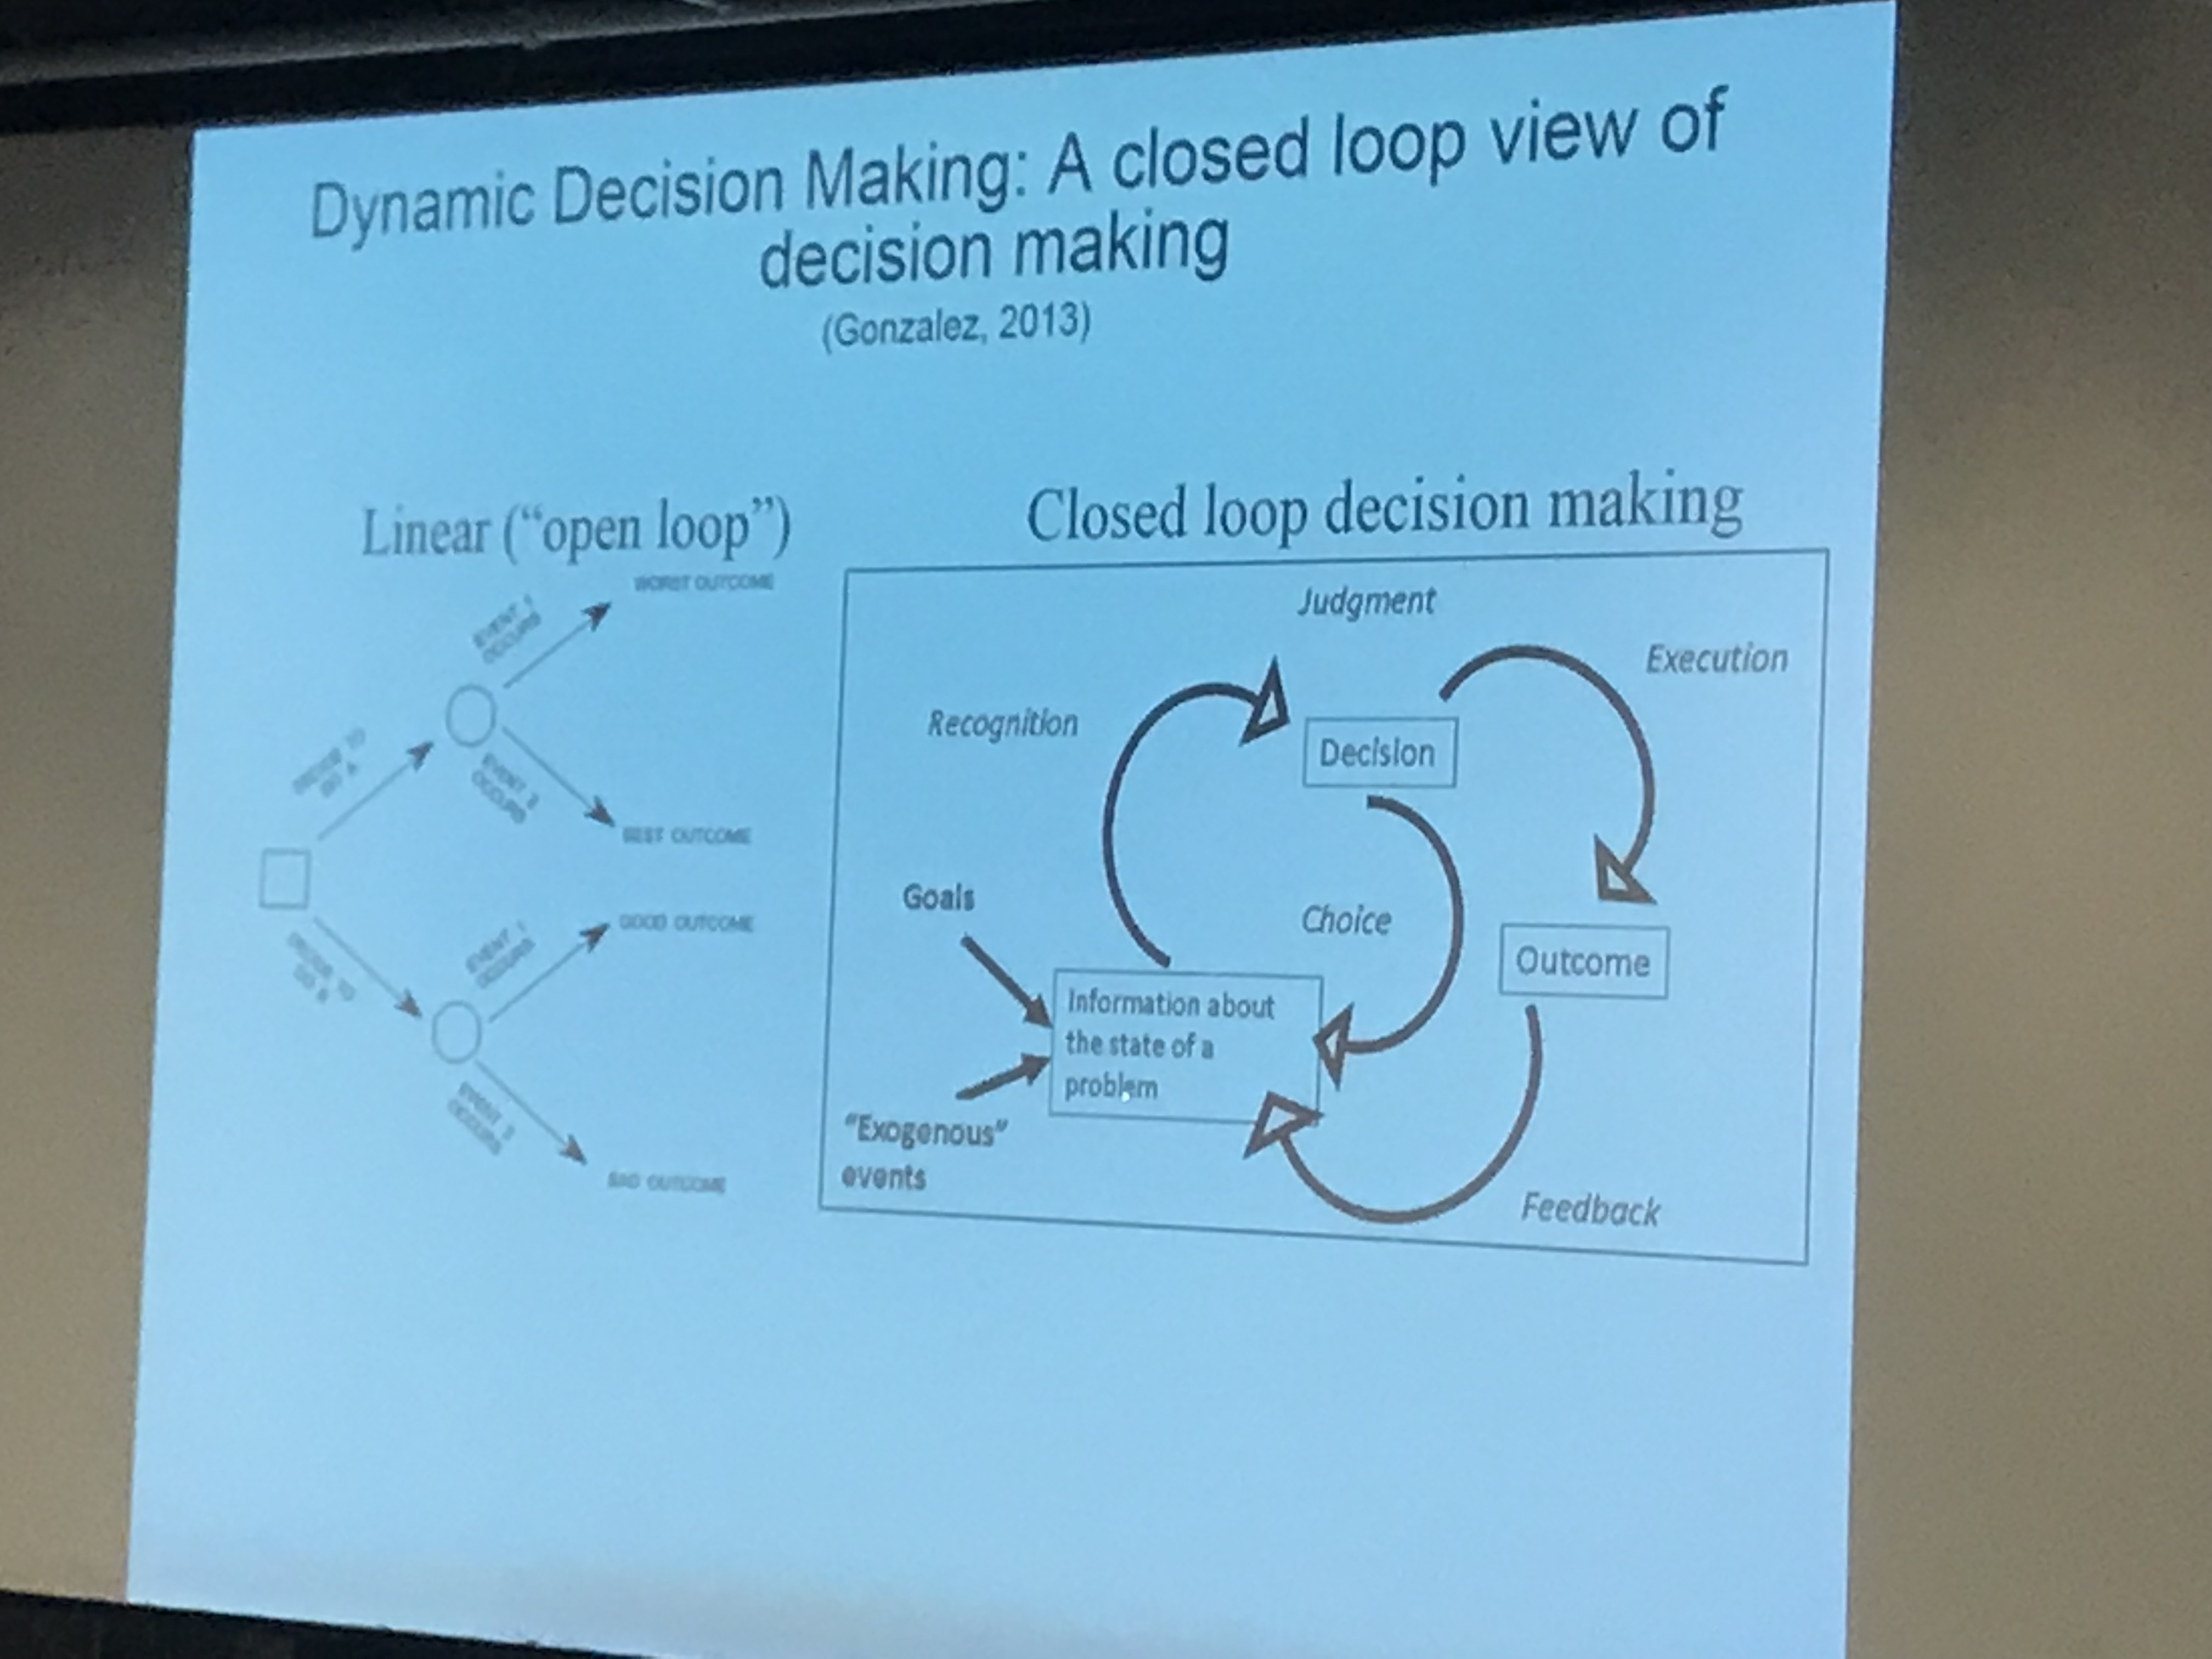
\includegraphics[width=0.55\textwidth]{images/ddm.JPG}
    \caption{Two extreme camps of decision making: classical decision theory (left) and naturalistic decision making/dynamic decision making (right)}
    \label{fig:ddm}
\end{figure}

\subsubsection{Dynamic Decision Making}

In a Dynamic Decision Making (DDM) problems:
\begin{itemize}
    \item Series of decisions over time
    \item Decisions are interdependent over time
    \item Environment changes
    \item Utility of decisions is time dependent
    \item Resources and time are limited.
\end{itemize}

Two types of DDM:
\begin{enumerate}
    \item {\bf Choice:} A series of choices under uncertainty in which goal is to maximize total reward over the long run.
    
    $\ra$ One style is to make decisions online and can't go back and redo them.
    
    $\ra$ Another is to try things out multiple times, sampling different strategies (as in trying different clothes before buying one).
    
    \item {\bf Control:} a series of choices under uncertainty in which the goal is to maintain a system in balance over time by reducing gap between a target and the actual state of the system.
\end{enumerate}

%Key aspect of any of these %decision making paradigms: learning! \\

$\ra$ Yields a continuum of dynamics in experimental tasks:
\begin{equation}
    \tx{Simple, dynamic tasks}\tx{----------------------------------} \tx{Complex, dynamic tasks}
\end{equation}

Lots of experimental study on {\it microworlds} used for studying decision making~\cite{difonzo1998microworlds}. \\

$\ra$ More recently, microworlds for studying fire fighting, medical diagnosis, climate change, real-time resource allocation, and so on~\cite{gonzalez2005decision,gonzalez2005use}. \\

Live demo! Showed the software of one of the microworld simulations: pumping water through a complex network to maximize amount of water sent. Emphasized the fact that decisions have to be made rapidly, in real time, with noise, delay, and so on. Key question is how people make decisions in these kinds of contexts. \\

Study from 2003~\cite{gonzalez2003instance}---explored three questions about people in DDM:
\begin{enumerate}
    \item Dose practice translate into better performance?
    \item Would practice under time constraints help to perform well?
    \item How do human abilities (intelligence, memory) influence making decisions in dynamic tasks?
\end{enumerate}

Experimental Findings: people under time constraints tend to follow heuristics more closely, whereas people given more time tend to move away from heuristics gradually and instead opt for making decisions based on contextual knowledge of the task (input-output relations). \\

Summary of findings from survey/experiments:
\begin{itemize}
    \item More practice under time pressure does not translate to best performance
    \item Practice with no time pressure can be more beneficial in future time limitations of same task
    \item Pattern matching abilities (as measured by Raven Progressive Matrices) can predict performance well
    \item People decrease use of simple heuristics with more practice in the task.
\end{itemize}

\subsubsection{How Do We Make Decisions in Dynamic Environments?}

Two key elements:
\begin{enumerate}
    \item {\it Recognition:} have I seen this before?
    \item {\it Experience:} Acquisition of context-specific knowledge with practice in a task yields input-output associations (roughly model-based predictions)
\end{enumerate}

More theories of learning in DDM by ~\citet{dienes1995role,gonzalez2003instance} and~\citet{gibson1997learning}, also ACT-R~\cite{anderson1997act}. \\

$\ra$ Explores computational models of DDM (see~\citet{gonzalez2003instance}). \\

Q: How general are these theories? Or are they fit to the tasks? \\

A: Claim is that these are picking up on generic theories of how decisions are really made. \\

$\ra$ Thus, a move back to simple dynamic tasks from the more complicated tasks. From water management-esque micro worlds to a much simpler ``beer game"~\cite{brunstein2010effects}. \\

Problem: The description-experience gap~\cite{hertwig2009description}. Consider the following:
\begin{itemize}
    \item Get \$4 with probability $0.8$, 0 otherwise, or get \$3 for sure. 
    \item Q: How do people make the decision given only this description, as opposed to having made a bunch of choices and learned these probabilities?
    
    $\ra$ People tend to overweigh rare event probabilities when read from the description, and tend to underweight the probability if learned from experience.
\end{itemize}


Q: How do people respond to rare events? \\

A: According to prospect theory, we have some inaccurate function of the probability of events in mind (overweight rare events, underweight likely, from description). But: ``theory is developed for simple prospects with monetary outcomes and state probabilities"~\citet{kahneman2013choices}. \\

Thus, motivates a new question: do these same phenomena occur when the decision maker comes to know the task through experience alone? \\

{\bf Summary:} DDM is an important frontier in understanding how people solve problems in the real world.

\spacerule

\subsection{Tutorial by Emma Brunskill: Counterfactuals and RL}

Example: a brief tale of two hamburgers! Consider two burgers, the $1/4$ pounder and the $1/3$ pounder. Marketing company thought the $1/3$ pounder would do really well.\\

$\ra$ But it failed! Because $3 < 4$, so people thought they were getting ripped off. \\

\subsubsection{RL for Education}

Q: Can we use RL methods to figure out how to teach people fractions? \\

A: Yes! Designed a game that uses RL to provide the right activity at the right time. It's RL because we track knowledge {\bf state} of student, and {\bf decisions} based on state (which activity do we provide next?) \\

$\ra$ 500,000 people have played this game. RL problem was given 11k learners' trajectories to learn a more effective strategy for maximizing student persistence. \\

Note: Long legacy of RL to benefit people. From bandit theory in 1940s to clinical trials. \\

What works in robotics and games: 1) we often have a good simulator, 2) enormous amount of data to train, 3) can always try out a new strategy in the domain. \\

$\ra$ In contrast, in working with people: 1) no good simulator of human physiology, and 2) Gathering real data involves real people and real decisions! \\

Big picture: interested in techniques to minimize and understand data needed to learn to make good decisions. \\

{\bf Background:} Usual story: an agent $\mathscr{A} : \mc{D} \ra \Pi$ outputs a policy given some history of data $D \in \mc{D}$, collected while interacting with an MDP $M = \langle \mc{S}. \mc{A}, R, T, \gamma \rangle$. \\

Counterfactual/Batch RL: we collect a dataset $D$ of $n$ trajectories $D_n \sim M(\pi)$. \\

Want to think about alternative ways to have made decisions based on this dataset. So, really: ``what if" reasoning given past data. \\

Challenging! For two reasons:
\begin{enumerate}
    \item {\bf Data is censored:} we don't know what existed in other universes (what if I didn't come to this universe?)
    \item {\bf Need for generalization:} almost always searching through an exponentially large space $|\Pi| = |\mc{S}|^{|\mc{A}|}$, or even infinite largely.
\end{enumerate}

Growing interest in Causal Inference and ML: see~\citet{pearl2018book} \\

Batch policy optimization: find a good policy that will perform well in the future:
\[
\underbrace{\argmax_{\pi \in \mc{H}_i} \max_{\mc{H}_i \in \{\mc{H}_1, \mc{H}_2, \ldots\}}}_{\tx{Policy Optimization}} \underbrace{\int_{s \in \mc{S}_0} \hat{V}^{\pi}(s, D) ds}_{\tx{Policy Evaluation}}
\]
The outer argmax and max are roughly policy optimization, with the inner integral roughly policy evaluation. \\

Q: What is our hypothesis class? \\

A: Could be lots of things! $\mc{H} = \mc{M}$? $\mc{H} = \Pi$? 
$\mc{H} = \mc{V}$?

\subsubsection{Policy Evaluation}

Q: How good is some alternative policy $\pi$, given data colllected from a previous policy, $\pi'$? \\

A: Huge literature, often from other communities! See treatment effect estimation from old data in economnetrics and biostatistics~\cite{rubin1997estimating}. \\

Q: Why is this problem hard? \\

A: Covariate shift! Under any policy, we can only see a small fraction of state-action space, so it's hard to get a sense of the rest of the domain from a single policy. See Figure~\ref{fig:cf} \\

\begin{figure}[h!]
    \centering
    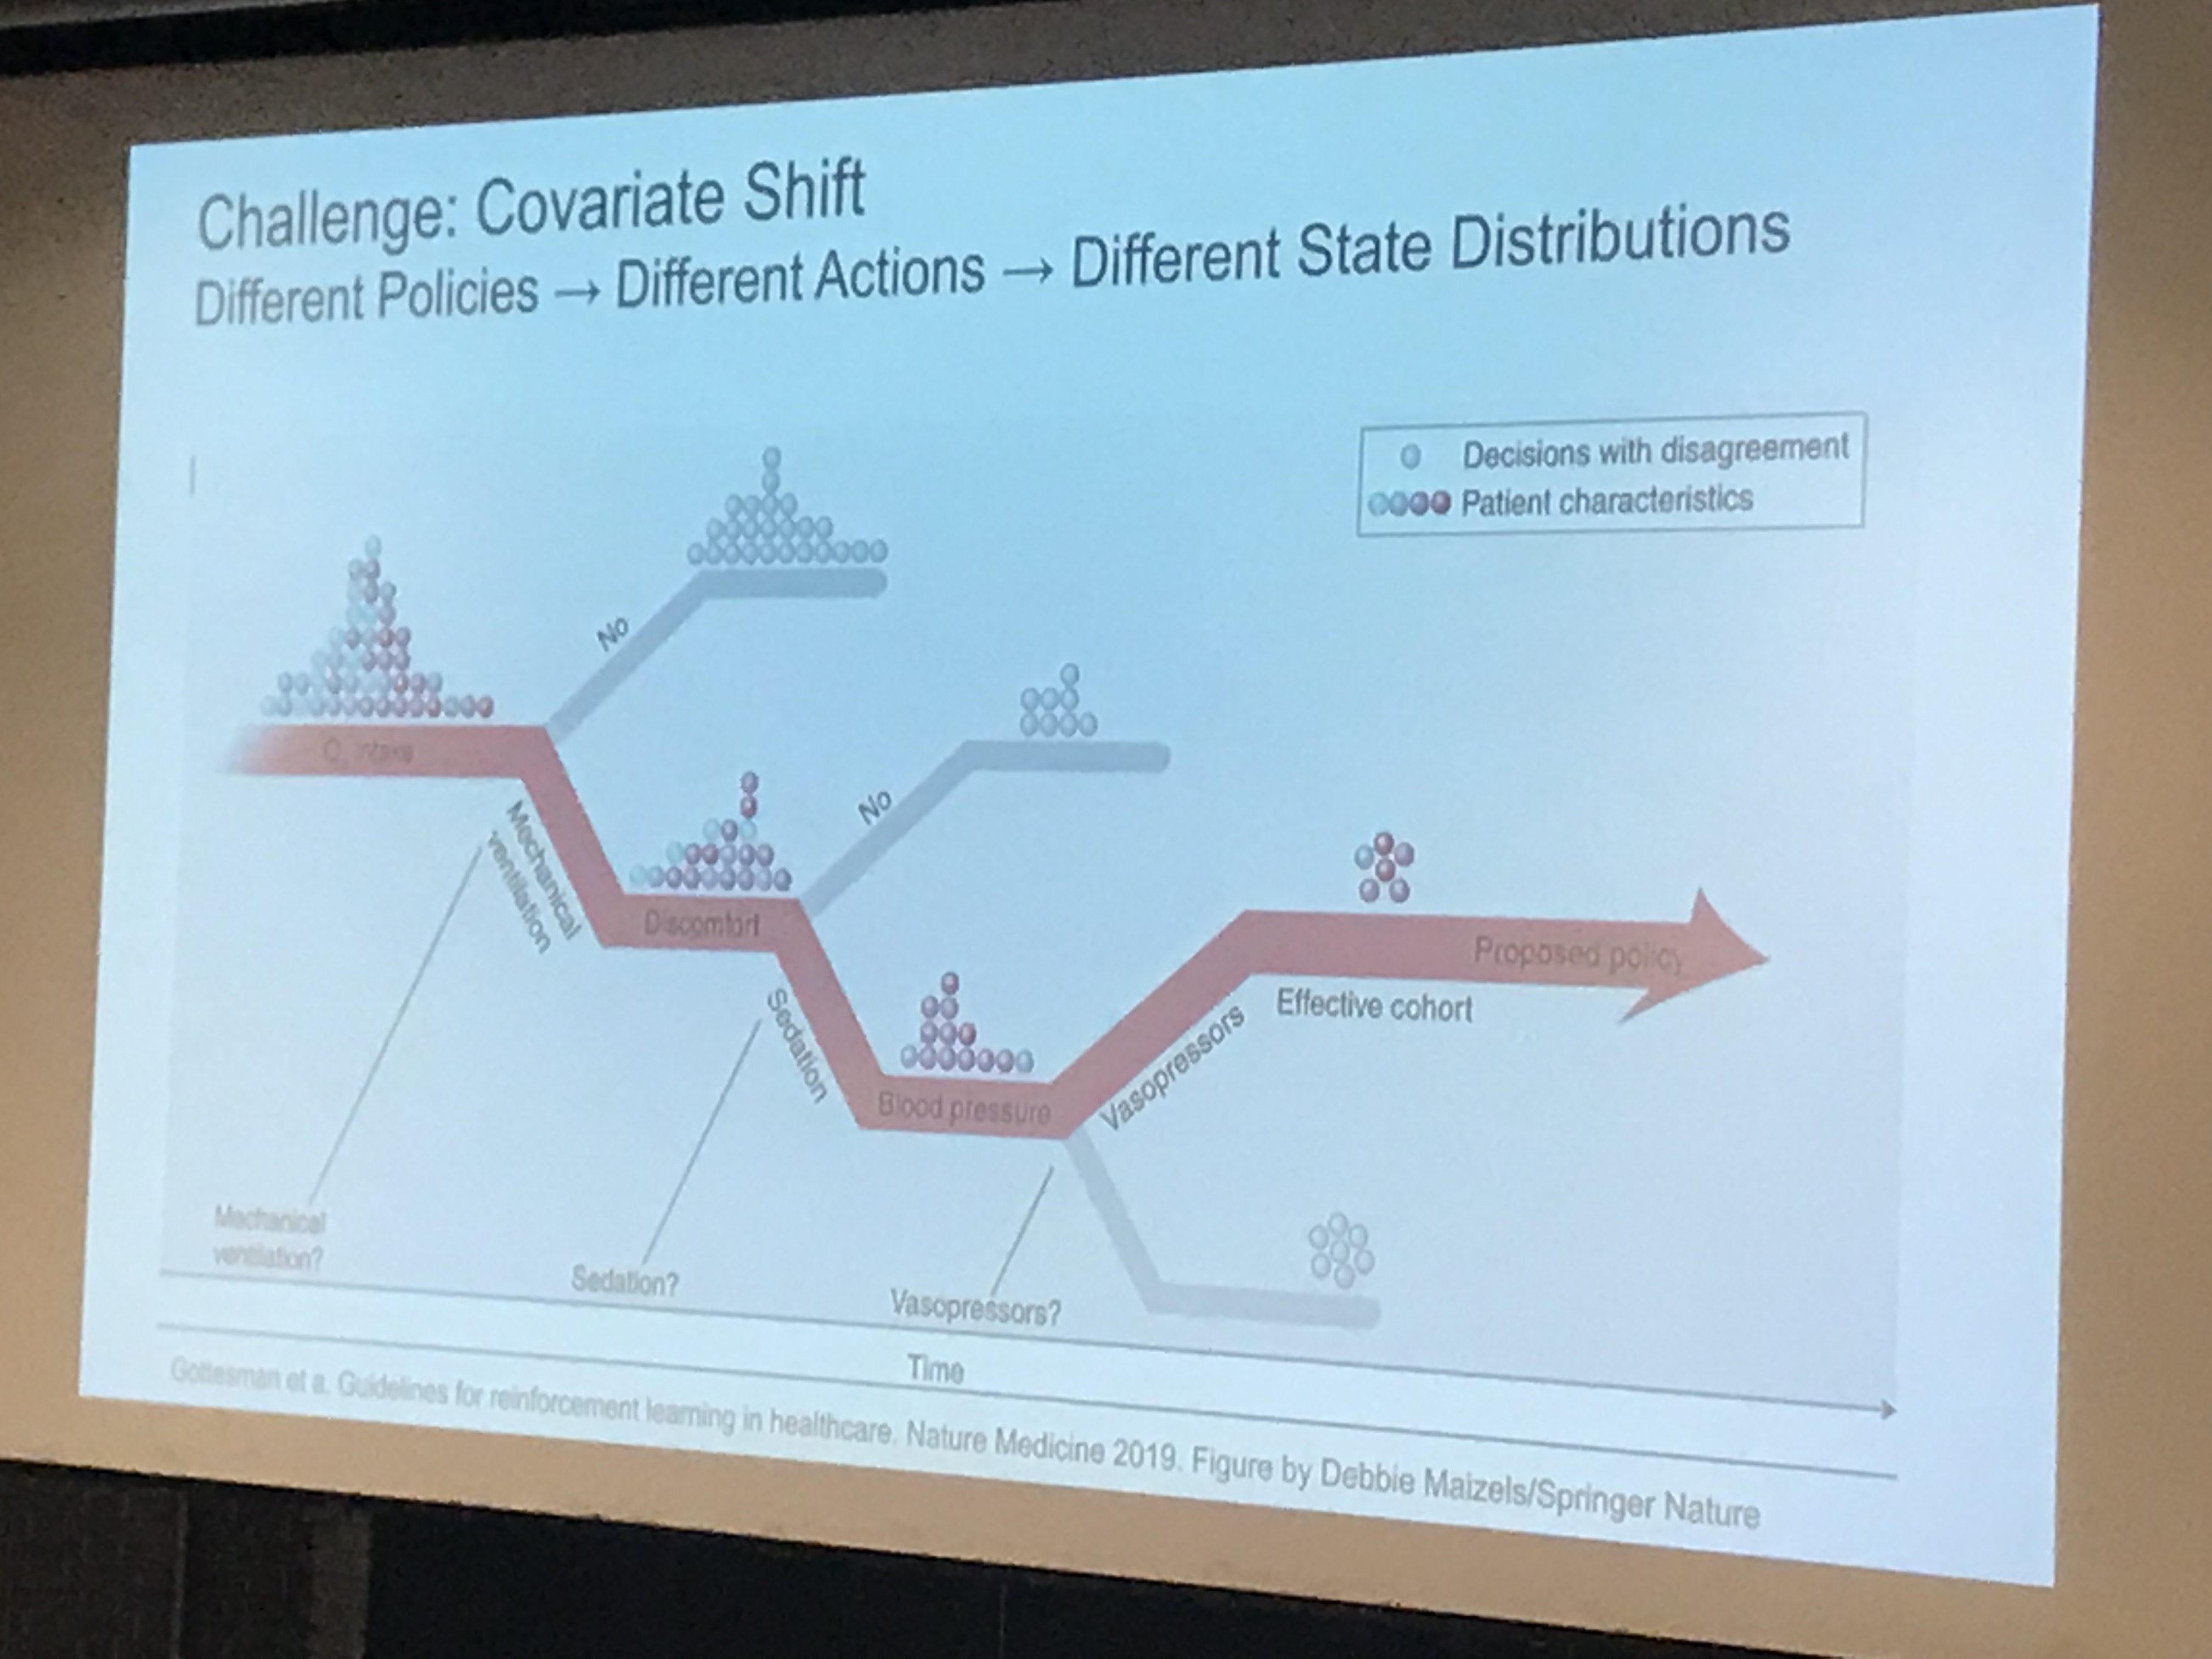
\includegraphics[width=0.5\textwidth]{images/cf.JPG}
    \caption{Covariate shift makes our effective data size very small.}
    \label{fig:cf}
\end{figure}

{\bf Idea 1:} Model-based policy evaluation:
\begin{align}
P^\pi(s' \mid s) &= p(s' \mid s, \pi(s)) \\
V^\pi &\approx (I - \gamma \hat{P}^\pi)^{-1}\hat{R}^\pi.
\end{align}
But: our model and reward function might be 1) wrong, 2) misspecified, 3) hard to estimate well. In any of these cases, these errors can compound and lead to a fundamental difficulty with using model-based methods. \\

{\bf Idea 2:} Model-free policy evaluation:
\begin{align}
    D &= (s_i, a_i, r_i, s_{i+1}),\ \forall_i \\
    \hat{Q}^\pi(s_i,a_i) &= r_i + \gamma V_\theta^{\pi}(s_{I+1})
\end{align}
Bias/variance trade-off lurking, depending on realizability of chosen hypothesis class. \\

$\ra$ Can overcome this using importance sampling:
\begin{align}
    V^{\pi}(s) &= \sum_\tau p(\tau \mid \pi, s) R(\tau) = \sum_\tau p(\tau, \pi_b, s) \frac{p(\tau, \pi, s)}{p(\tau \mid \pi_b, s)} R(\tau) \\
    &\approx \nsum \frac{p(\tau_i, \pi, s)}{p(\tau_i \mid \pi_b, s)} \\
    &= \nsum R(\tau_i) \prod_{t=1}^{H_i} \frac{p(a_{it} \mid \pi, s_{it})}{p(a_{it} \mid \pi_b, s_{it})}.
\end{align}

But, this approach is all trajectory based. Might also right this down in terms of state-actions (so replace $p(\tau \ldots)$ with a distribution over state-action pairs, might come from stationary distribution). \\

\begin{figure}[h!]
    \centering
    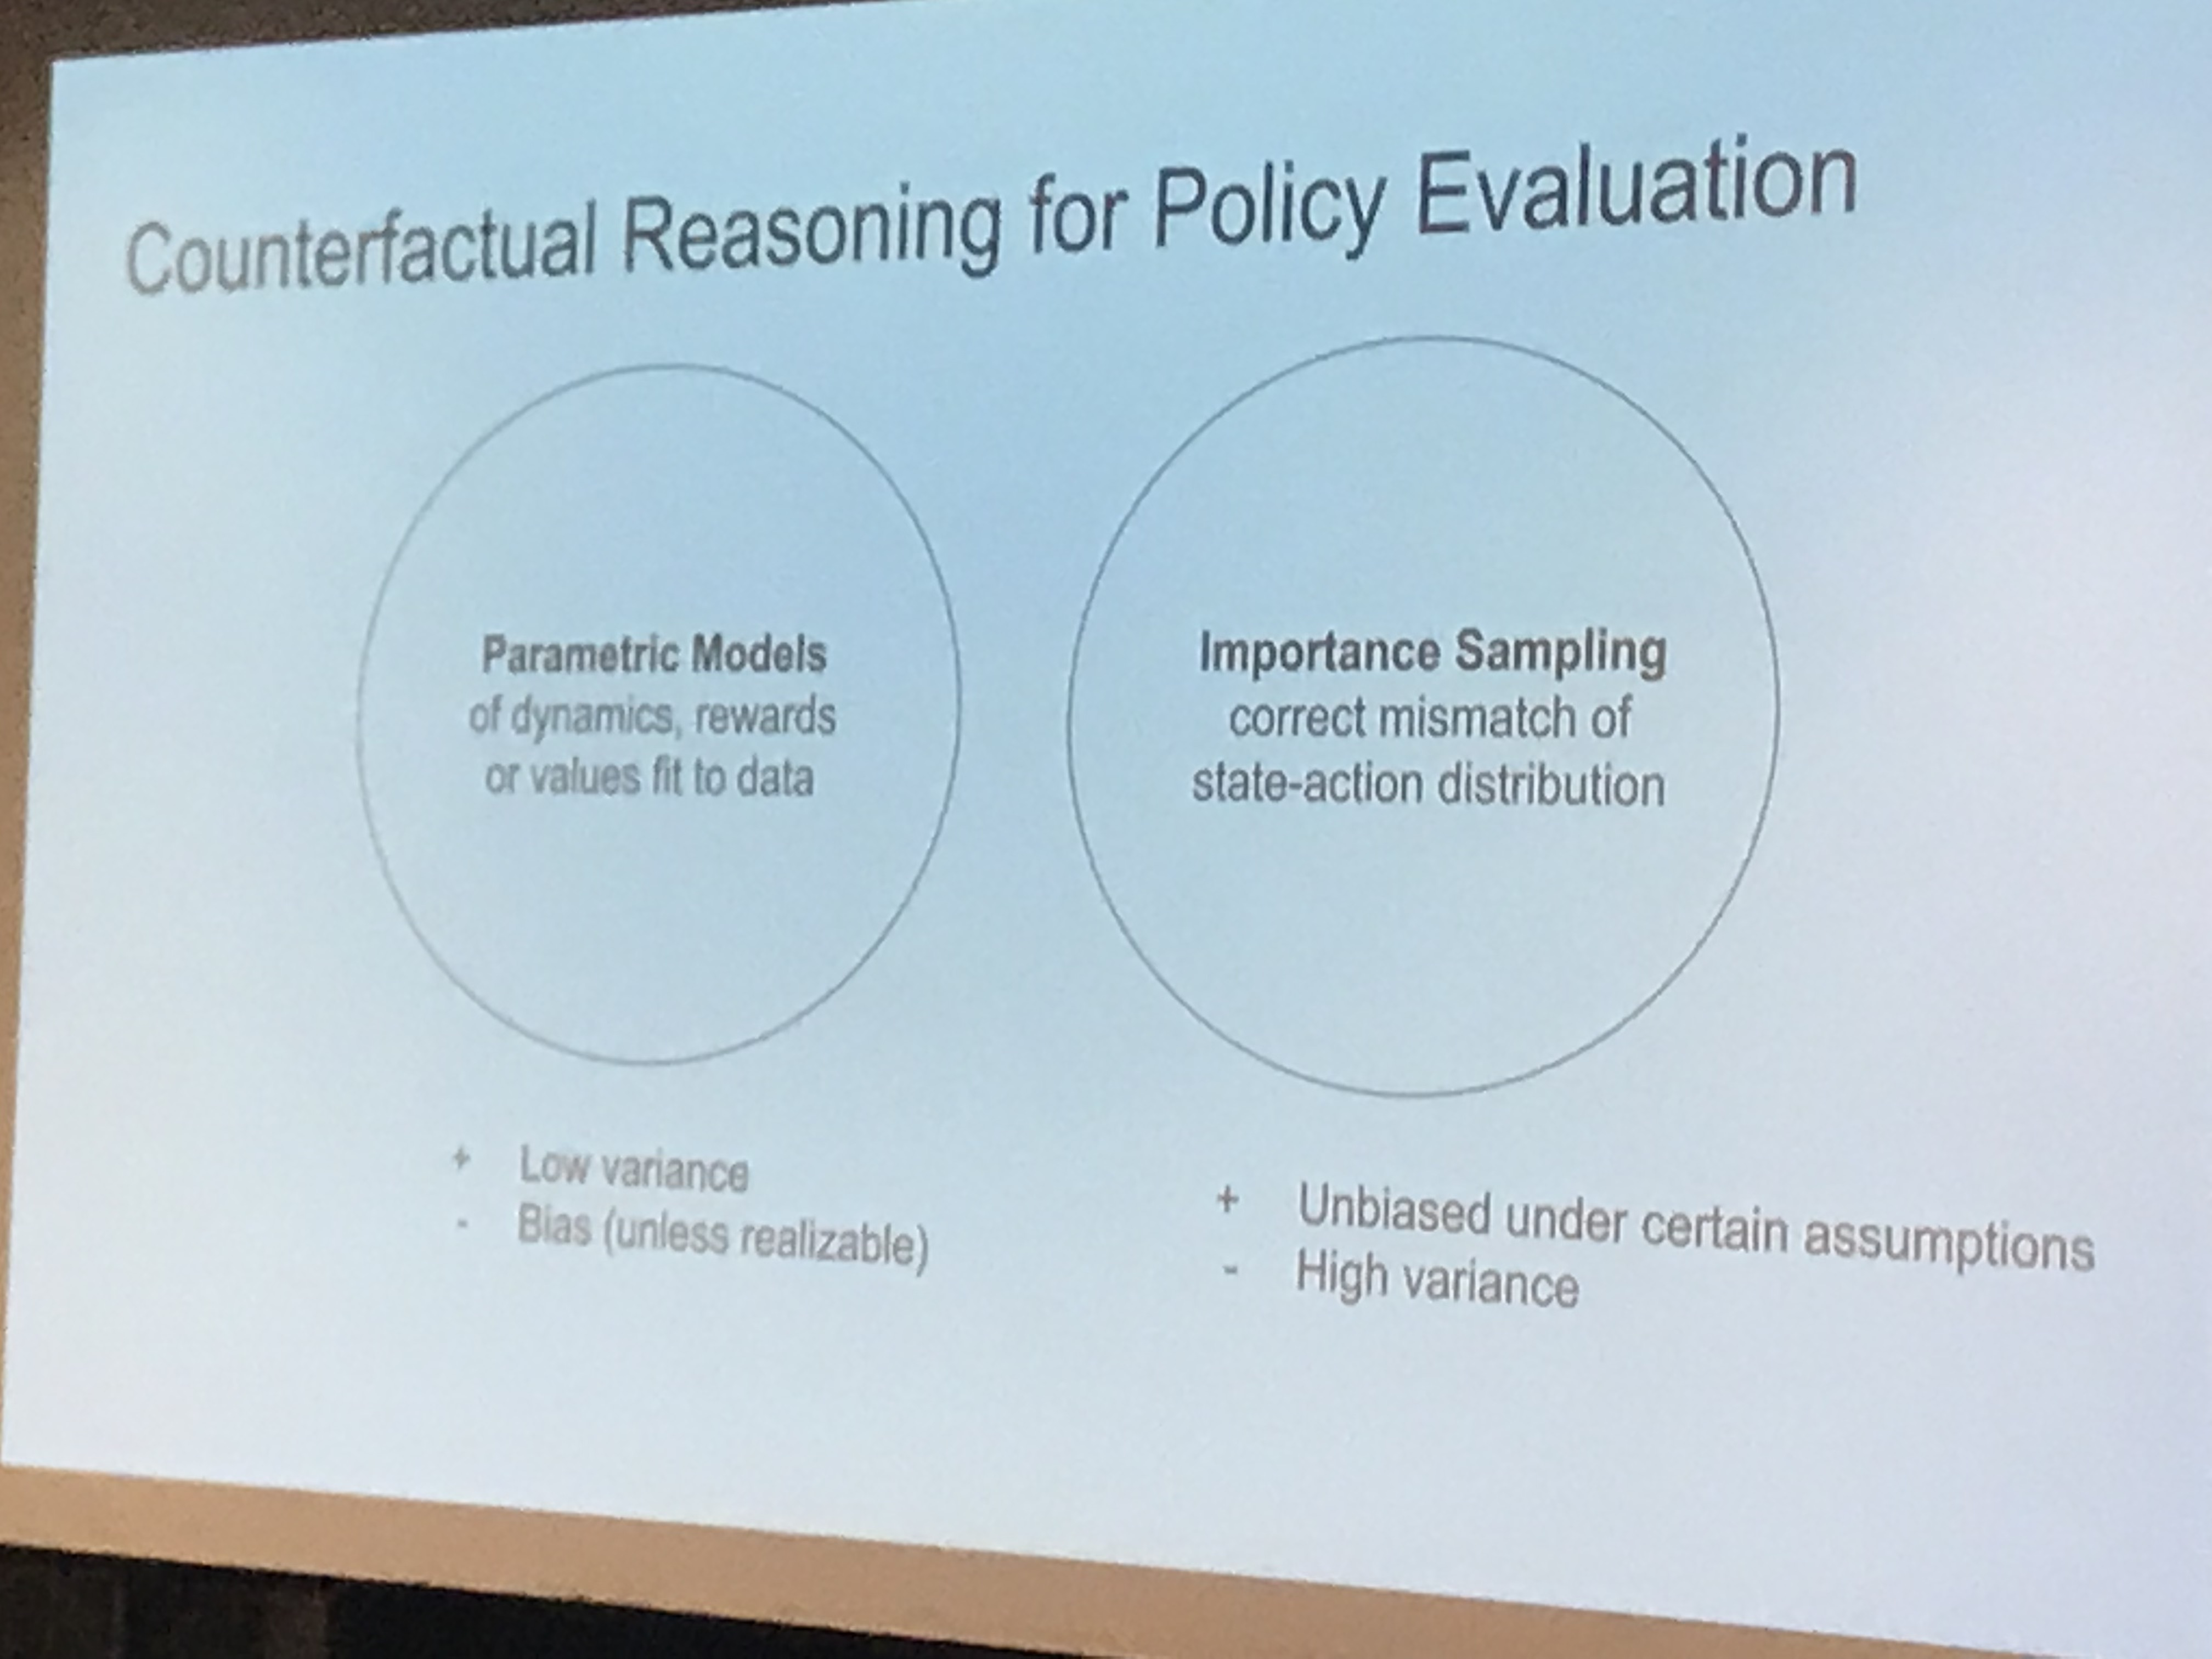
\includegraphics[width=0.4\textwidth]{images/pv.JPG}
    \caption{Pros and Cons of two approaches to off-policy evaluation}
    \label{fig:pv}
\end{figure}

So, two approaches (See Figure~\ref{fig:pv} for comparison). Can we combine the two nice properties? \\

A: Yes! The doubly robust estimator in bandits~\cite{dudik2011doubly}, then extended to RL~\cite{jiang2015doubly}:
\begin{align}
DR(D) &:= \nsum \sum_{t=0}^\infty \gamma^t w_r^i R_t^{H_i} + \ldots
\end{align}

Note: most of these estimators are about making different bias/variance trade-offs. \\

Two new off policy evaluation estimators;
\begin{enumerate}
    \item Weighted doubly robust for RL~\cite{thomas2016data}: weighted importance sampling leads to lower variance.
    \item Model and Guided Importance Sampling: how much should we weight each kind of estimator? Solve this with a quadratic program, yield a reasonable bias/variance trade off.
\end{enumerate}

But! We don't know the target: if we could actually evaluate the bias, we would already know the true value. So, how can we approximate the bias? \\

$\ra$ In general, very hard. But, we might be able to get a conservative estimate of the bias $\ra$ use confidence intervals around the importance sampling estimate to bound the bias. \\

Huge caveat, though, for applying these ideas to healthcare applications: we don't really know the true behavioral policies of medical practitioners! Almost all observational health data has this issue (and others: state data we don't have access to, etc.). \\

Summary:
\begin{itemize}
    \item Model-based approach and Model-free approach, but each make trade offs
    \item Importance sampling is crucial!
    \item Double robust methods try to take the best from both sides.
\end{itemize}


\subsubsection{Policy Optimization}

Q: Now, given that we can evaluate a policy, how do we improve policies? \\

A: Lots of approaches! One early idea introduce by \citet{mandel2014offline}: finding was that the best model for {\it making decisions} was different from the model that was best for {\it prediction}. Lots of confounding factors (approximate model, limited data, overfitting, and so on). \\

Consider {\it fairness} of these estimators: an estimator is unfair if it chooses the wrong policy more than $1/2$ of the time. \\

$\ra$ Can show that even if importance sampling is unbiased, policy selection using them can be unfair. Problem is having different variance across different estimators! \\

{\bf Grand quest in RL:} how do we do structural risk minimization for RL? We {\it do not} have an answer for this yet. \\

For example, we would llike to be able to include a hypothesis-class complexity term capturing our generalization error, like VC-dimension:
\[
\underbrace{\argmax_{\pi \in \mc{H}_i} \max_{\mc{H}_i \in \{\mc{H}_1, \mc{H}_2, \ldots\}}}_{\tx{Policy Optimization}} \underbrace{\int_{s \in \mc{S}_0} \hat{V}^{\pi}(s, D) ds}_{\tx{Policy Evaluation}} - \underbrace{\sqrt{\frac{f(\tx{VC}(\mc{H}_i) \ldots)}{n}}}_{\tx{Error Bound}}
\]

Some ideas: look to FQI, model-free batch RL, importance sampling bounds, primal dual approaches, Tend to assume realizability, though. \\

Aim: strong generalization guarantees on policy performance.  \\

Super hard! Lets instead focus on just finding a good policy in a policy class. \\

New result: can probably converge to local solution with off policy batch policy gradient~\cite{liu2019off}. \\

$\ra$ Has implications for online learning, too. (Basically: we can use our data better.) \\

Next up: can we guarantee we find the {\it best policy} from a given class, and to guarantee how far we are from the best solution:
\[
\max_{\pi \in \Pi} \int_s V^\pi ds - \int_s V^{\hat{\pi}}(s) ds \leq \sqrt{\frac{f(\ldots)}{m}},
\]
where the complexity term of the hypothesis class is instead an entropy based term. For details see work by~\citet{nie2019learning}. \\

Main idea: use an advantage decomposition. So:
\[
\Delta_\pi := V_\pi - V_0 = \bE_0 \left[\nsum \indic\{\mu_{\tx{now}}(s_i) - \mu_{\tx{next}}(s_i)\}\right].
\]
Comes from~\citet{kakade2003sample,murphy2005generalization}. \\

Q: Does this work empirically? \\

A: In healthcare tasks, yes! For large amounts of data, achieves extremely low regret relative to other estimators. \\

{\bf Summary:}
\begin{itemize}
    \item Open and active quest for Bath policy optimization with generalization guarantees. We need an SRM theory for RL!
    
    \item This is a really, really hard problem in general! But, some optimism: from the education case in the beginning (teaching people fractions), it actually worked!
    
    \item Q: How does this relate to exploration?
    
    Some early answers from~\citet{tu2018gap} and \citet{sun2018model}.
    
    
\end{itemize}



\spacerule



